This section is a refinement of the chapter "3.1.1 User Interface" of the Requirements Analysis and Specification Document (RASD) related to the \app project.
At the level of detail that is allowed for a design document, it is possible to delve deeper into the various interactions that the platform offers to the external user (either a student or an educator). 

The images inserted in this section serve as mockups of the user interfaces provided by the system and therefore they have to be interpreted as general guidelines for the designers and developers to grasp the application should look like at the end of the implementation process. 

In order to facilitate the understanding of the reader, the following description is going to take first the point of view of an Educator using \app and then there will be a switch to the student perspective.

\subsection{Login Phase}
The initial step for accessing \app is of course logging in the system, and this is possible thanks to the initial user interface provided by the application. It is illustrated in the following image:

\begin{center}
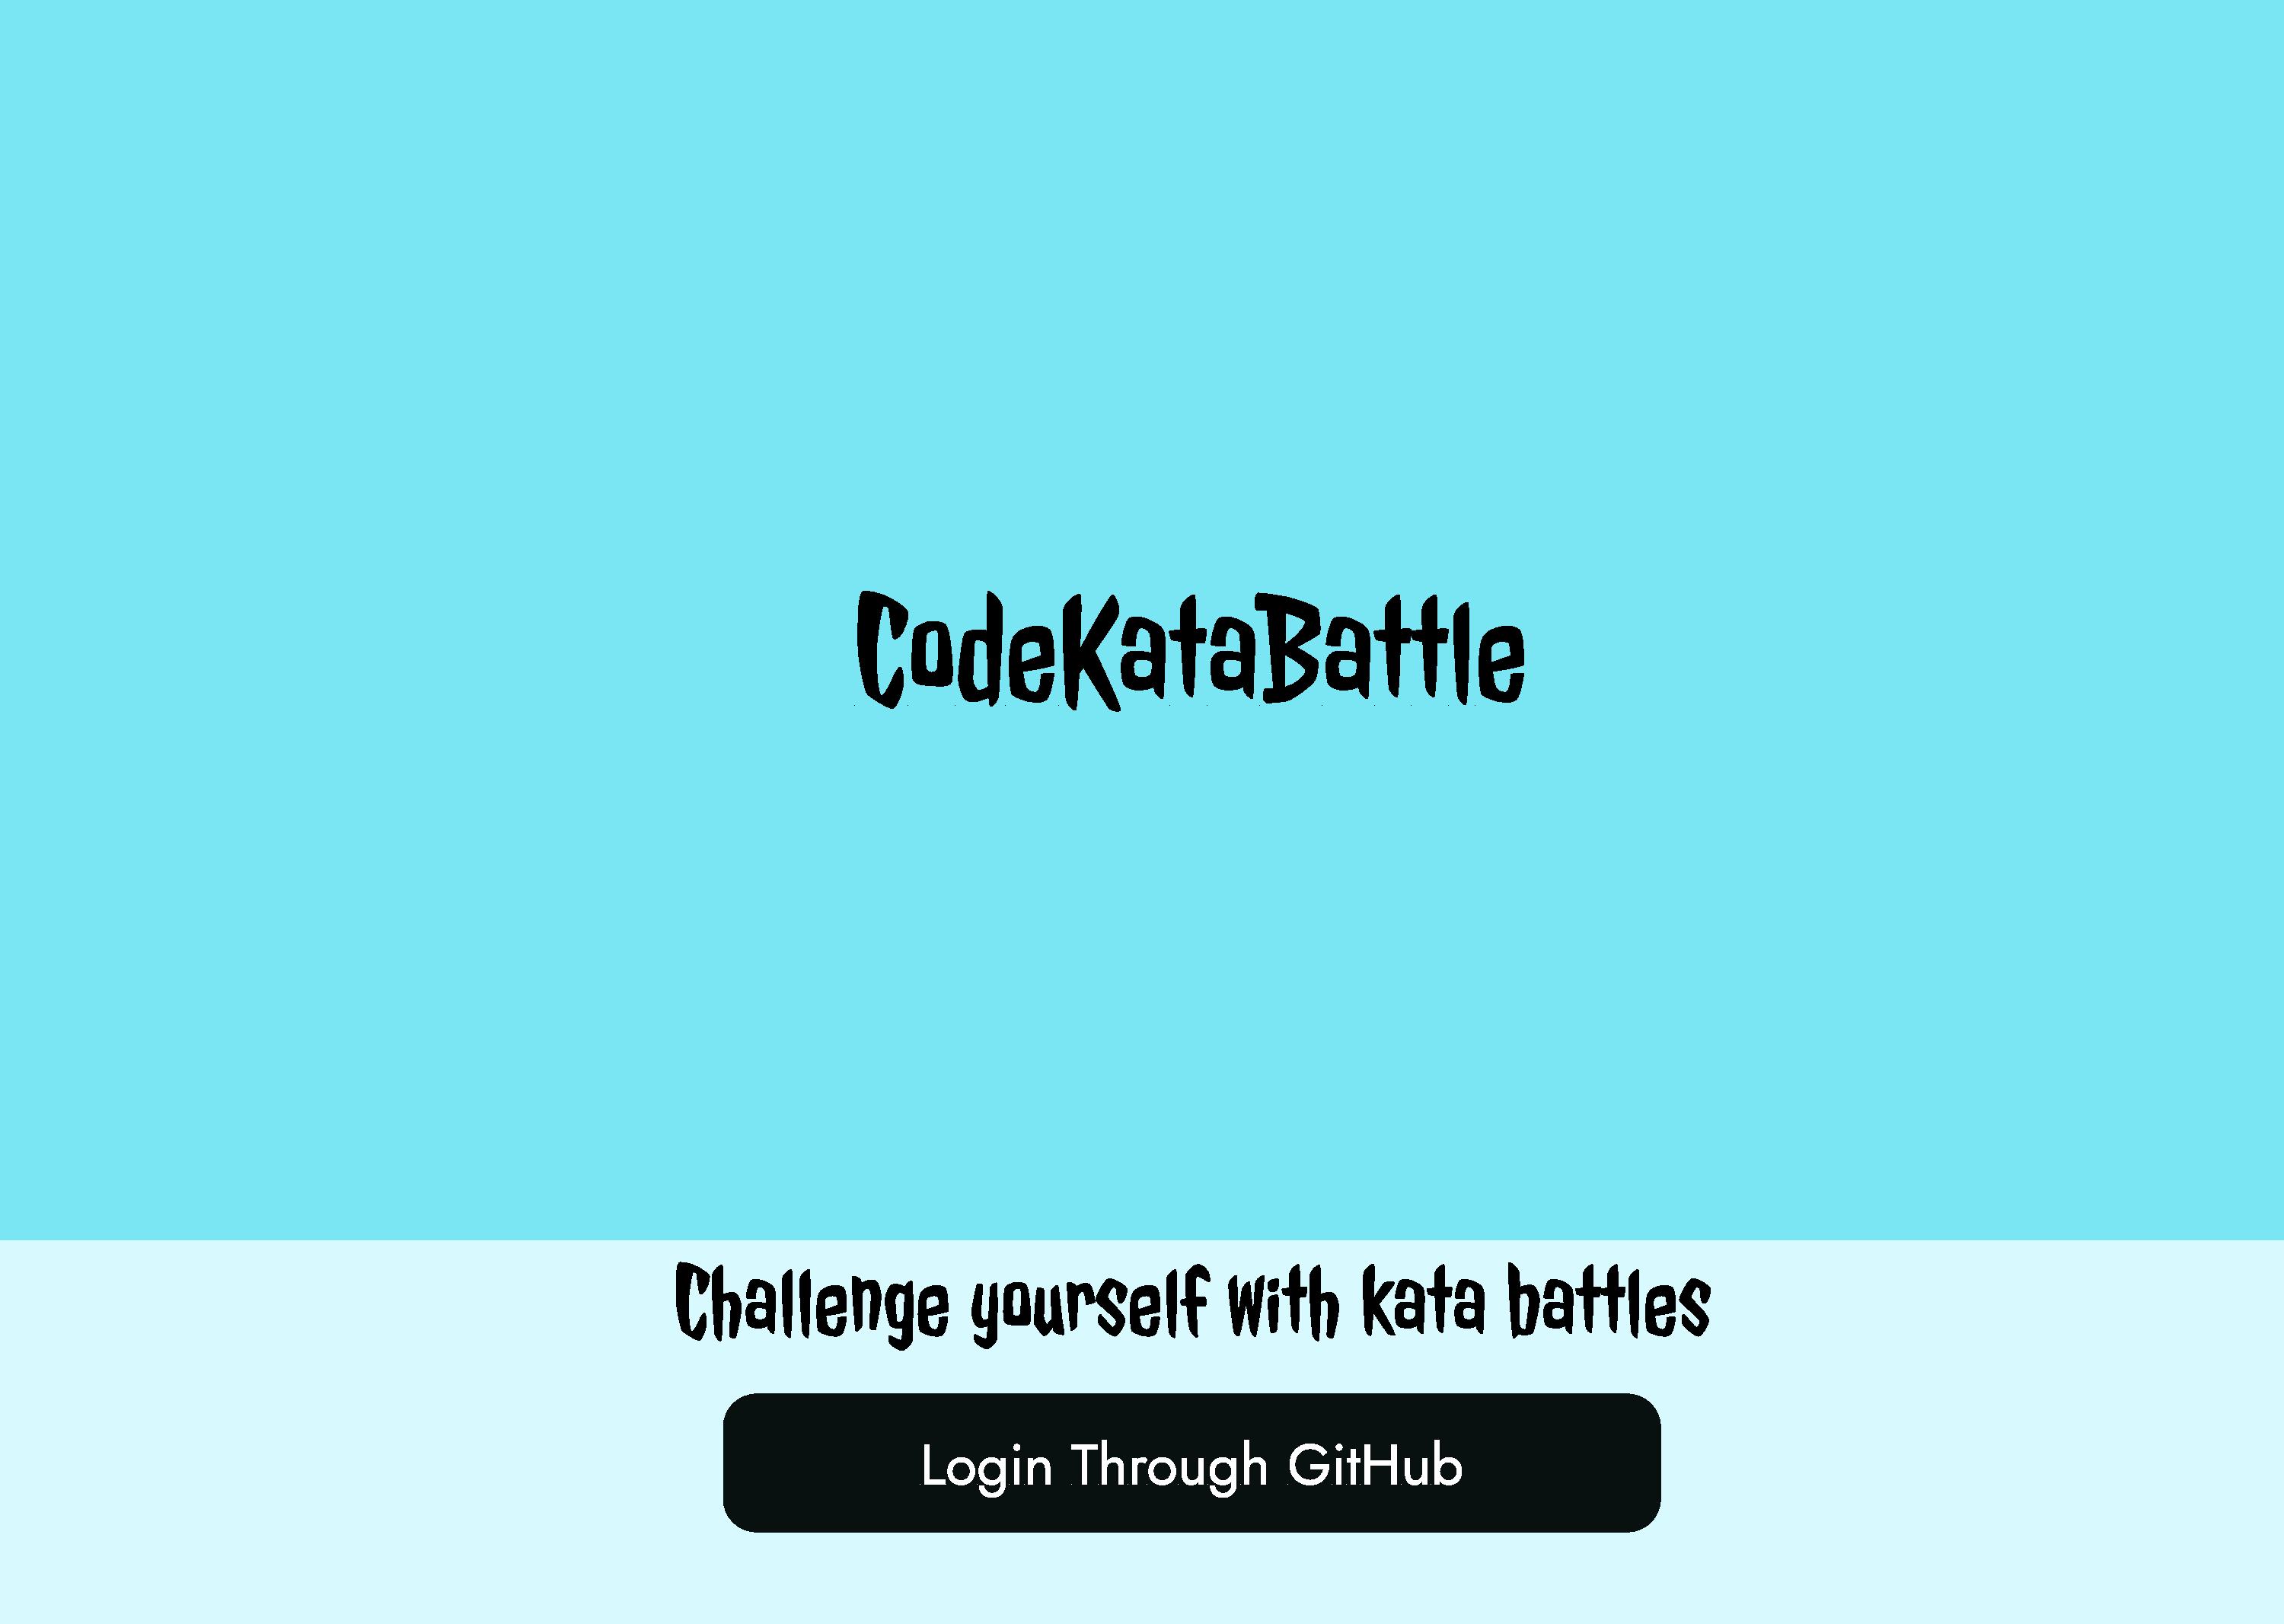
\includegraphics[width=0.8\linewidth,page=1]{MockupUI}
\end{center}

By clicking on the button "Login Through Github" the user will be redirected to a web page where s/he will be able to insert his/her personal GitHub credentials.

\begin{minipage}{\linewidth}
\subsection{Educator personal profile}
As stated in the introduction, the description now takes the point of view of an educator.
The first page displayed after the login is the personal profile of the educator, as it is possible to observe in the following illustration:

\begin{center}
	\includegraphics[width=0.8\linewidth,page=3]{MockupUI}
\end{center}

\end{minipage}

This page offers various functionalities:
\begin{itemize}
	\item My Tournaments button allows an educator to see the list of tournaments that s/he created or the ones s/he has permissions to publish battles in. The Tournament microservice is responsible for providing this list.
	\item New Battle button allows for the creation of a new battle. When the educator clicks on it, the Tournament microservice is involved because a list of tournaments in which the educator is allowed to publish battles has to be supplied. The educator is then able to select a tournament out of that list (in which s/he wants to publish the battle) and automatically the page for creating the new battle pops up (as described later on).
	\item New Tournament button allows for the creation of a new tournament. The request is passed to the Tournament Microservice which will reply with the tournament creation form (as shown later on).
\end{itemize}

Let's assume now the educator clicks on the "New Tournament" button. The following section shows the interface that pops up in this case.

\begin{minipage}{\linewidth}
\subsection{Creation of a new tournament}
In order to create a new tournament, the tournament creation form has to be filled in by the educator. A sketch of how this form would look like is reported here:

\begin{center}
	\includegraphics[width=0.8\linewidth,page=4]{MockupUI}
\end{center}

\end{minipage}

The most important pieces of information for a tournament are clearly visible in the image, as the educator is able to set the tournament name, the tournament description and the registration deadline. There is also a dedicated section for the badges, that will be assigned at the end of the tournament.

Once the educator fills in all the form, s/he can confirm with the button in the bottom right side of the interface. As s/he does it, the tournament home page appears on the screen, as illustrated in the next section.

\begin{minipage}{\linewidth}

\subsection{Tournament home page}
Whenever a student or an educator search for a tournament and clicks on it, the tournament home page pops up. This is how the page is designed in order to provide all the relevant information related to a tournament:

\begin{center}
	\includegraphics[width=0.8\linewidth,page=6]{MockupUI}
\end{center}

\end{minipage}

In the top right corner of the page, there is a button that allows the user to join the tournament. As a student clicks on it, the request is dispatched to the Tournament Microservice that will take care of verifying if the registration deadline for the tournament hasn't passed yet and consequently add the student to the set of students subscribed to the tournament.

On the left, a list of the battles published within the tournament are available for students to join them and for educators to see them. 
On the right hand side, two panels appear. Going top to bottom, the first one is a list of battles that the student joined, the second one is the tournament ranking, which displays all the students participating in the tournament as a list of names.


\begin{minipage}{\linewidth}

\subsection{Creation of a new battle}

Let's now go back to the educator's home page (educator profile). Let's suppose the educator clicks on the "New Battle" button. The first response of \app will be showing a list of the tournaments in which the educator has permissions to publish battles. The following image shows this interface:

\begin{center}
	\includegraphics[width=0.8\linewidth,page=10]{MockupUI}
\end{center}

\end{minipage}

As the educator selects the tournament, a new page shows up, displaying the battle creation form.

\begin{center}
	\includegraphics[width=0.8\linewidth,page=5]{MockupUI}
\end{center}

All the pieces of information that are needed for the creation of a new battle have their respective fields in this user interface. Once all these parts have been correctly defined, the educator can confirm his/her choices with the button in the bottom right corner of the interface. 
As the confirmation button is pressed, the Battle Microservice will be immediately provided with all the data that the educator provided through this interface, in order to allow the Battle Manager to create a new battle and store this data in a persistent manner.

It is now possible to switch to the student's point of view to illustrate the user interfaces that the \app system provides.

First off, the interface for signing in \app is the same, as both educators and students are required to log in through their GitHub account.

\subsection{Student personal profile}
As the login phase is successfully concluded \app displays the student's personal profile. The following figure sketches the look of this user interface:

\begin{center}
	\includegraphics[width=0.8\linewidth,page=2]{MockupUI}
\end{center}

In the central part, a list of the badges earned by the student is shown, and it is visible to all the users of \app navigating to this student's profile.
The buttons on the right hand side offer the major functionalities that the student requires in order to use the application.

When the student clicks on the "Notifications" button, \app responds with a new interface that shows all the notifications that arrived for the student in question. The Notification Microservice is responsible in this case for retrieving the list of notifications related to a specific student and building the corresponding interface, which is shown in the following section.


\begin{minipage}{\linewidth}
\subsection{Notification interface}
Here's a mockup of the Notification interface for a student:

\begin{center}
	\includegraphics[width=0.8\linewidth,page=9]{MockupUI}
\end{center}

\end{minipage}

The illustration is pretty straightforward as it is composed of a single central pane that gathers all the notifications for the student. Among the various notifications that can reach a student there are:
\begin{itemize}
	\item Notification for the creation of a new tournament.
	\item Notification for the request of another student to join a battle together as a team.
	\item Notification for the creation of a new battle.
	\item Notification that carries the link to the remote GitHub repository for a battle the student is subscribed to.
	\item Notification for the termination of a tournament.
	\item Notification for the termination of a battle.
\end{itemize}

Going back to the student's personal profile, let's see what happens when the "Join Tournament" button is clicked. 


\begin{minipage}{\linewidth}

\subsection{Joining a tournament}
As the "Join Tournament" button is clicked, \app provides to the student a list of tournaments that are available in that moment inside the platform. The Tournament Microservice is responsible for providing such list of tournaments and building the relative user interface.

This is the look of the interface for joining a new tournament:

\begin{center}
	\includegraphics[width=0.8\linewidth,page=7]{MockupUI}
\end{center}

\end{minipage}

The student can browse all the tournaments available on \app from here. When the student clicks on one of the tournaments, the tournament home page shows up (as illustrated in section 3.4) and the button "Join Tournament" will be visible if the registration deadline for the tournament hasn't passed yet.


\begin{minipage}{\linewidth}
\subsection{Joining a Battle}
In order to join a new battle, the student has to start from his personal profile and click on the button "My Tournaments". The Tournament Microservice will be queried as a consequence and a list of tournaments to which the student is subscribed is displayed. This step is necessary because it is not possible to subscribe to a battle in a tournament without having previously joined the tournament itself.
From the list of tournaments, the student will select the one in which s/he wants to join a battle, and the tournament home page will pop up. The tournament home page contains the list of battles for that specific tournament. From here, the student can browse all the battles available. When s/he clicks on one of these battles, the battle home page is shown.
The following image gives a representation of the battle home page:

\begin{center}
	\includegraphics[width=0.8\linewidth,page=8]{MockupUI}
\end{center}

\end{minipage}

In the top right corner, the button to join the battle is displayed if the battle's registration deadline hasn't passed yet. 
In the left hand side, the battle description is provided, to make the student understand what kind of coding challenge the battle focuses on. On the right hand side, there is a list of scores associated to the student's code solutions for that battle (initially empty) and the battle ranking (ranking of teams).
